\section{Background of DDoS attacks}
\label{sec2}

A \gls{dos} attack aims to disrupt the service delivery of a system and as a result limits the
utility of the system for legitimate users \cite{specht2004distributed}. A \gls{ddos} attack
utilises several compromised machines to each perform a coordinated \gls{dos} attack against a single
target. This amplifies the effectiveness of the \gls{dos} attack, and helps mask the origin of the
attack. The machines used to perform the \gls{dos} attack on the target are usually compromised
machines which perform the coordinated attack based on the instructions from a handler. This
attack architecture is commonly referred to as the \gls{ddos} Agent-Handler Attack Model and is
depicted in Fig.~\ref{fig:Chap2_DDoS_Model}. In this architecture, the attacker
controls one or more handler which each control several agents (or compromised machines). The
attacker uses the handlers to coordinate the attack amongst all of the compromised hosts and in so
doing, amplifies the effectiveness of the \gls{dos} attack. This attack architecture is usually
associated with botnets.

\begin{figure}[h]
    \centering
    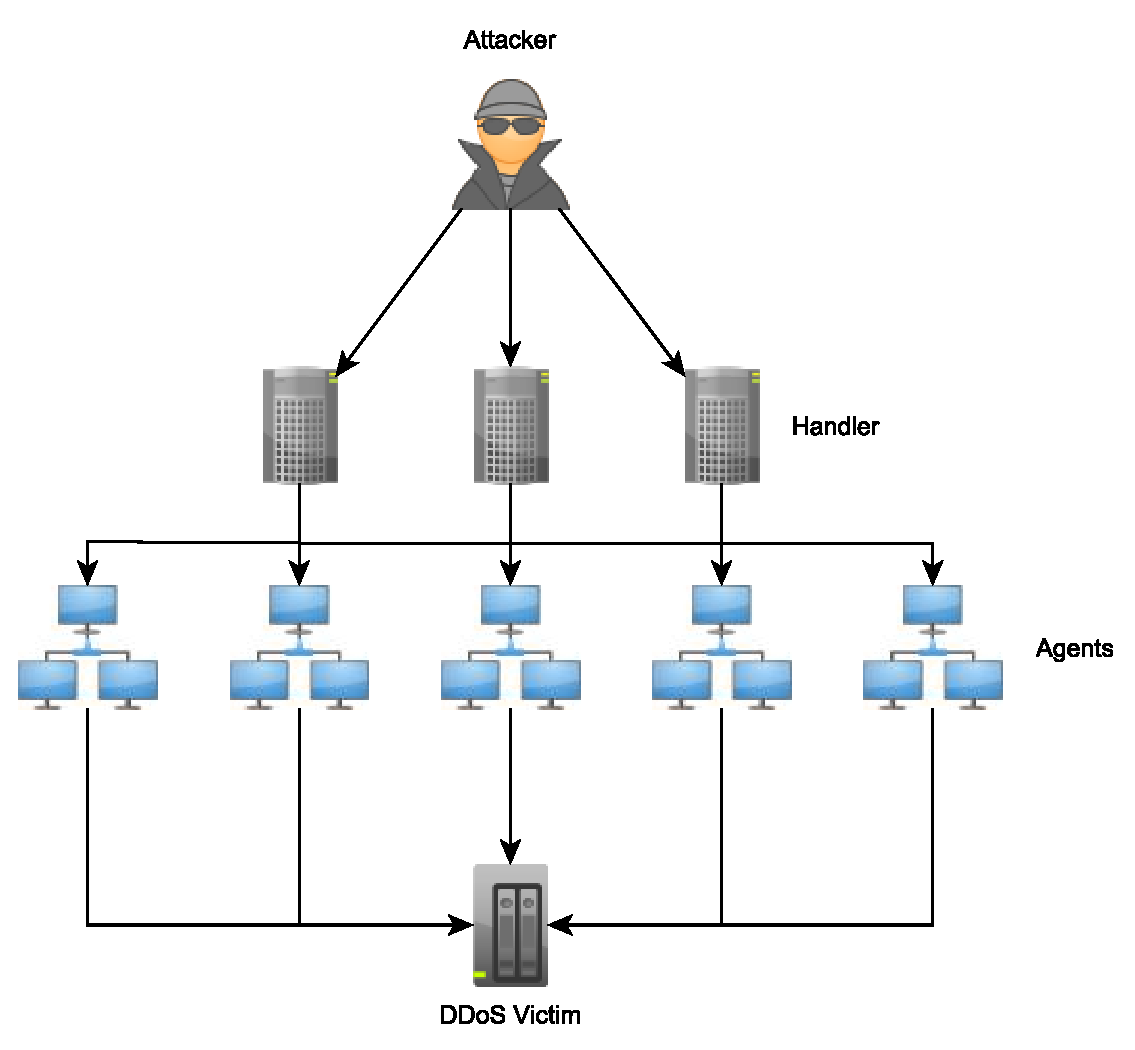
\includegraphics[width=\columnwidth]{section_2/Agent_Handler_Arch.eps}
    \caption{\gls{ddos} Agent-Handler Attack Model}
    \label{fig:Chap2_DDoS_Model}
\end{figure}

Specht  \textit{et al.}  \cite{specht2004distributed} created a \gls{dos} taxonomy to help classify various \gls{dos} attack
methods.  The taxonomy is depicted in Fig.~\ref{fig:Chap2_DDoS_Tax}.
According to Specht  \textit{et al.}\cite{specht2004distributed}, there are two primary classes of \gls{ddos}, namely \textit{bandwidth depletion} and \textit{resource depletion}.

\begin{figure}[h]
    \centering
    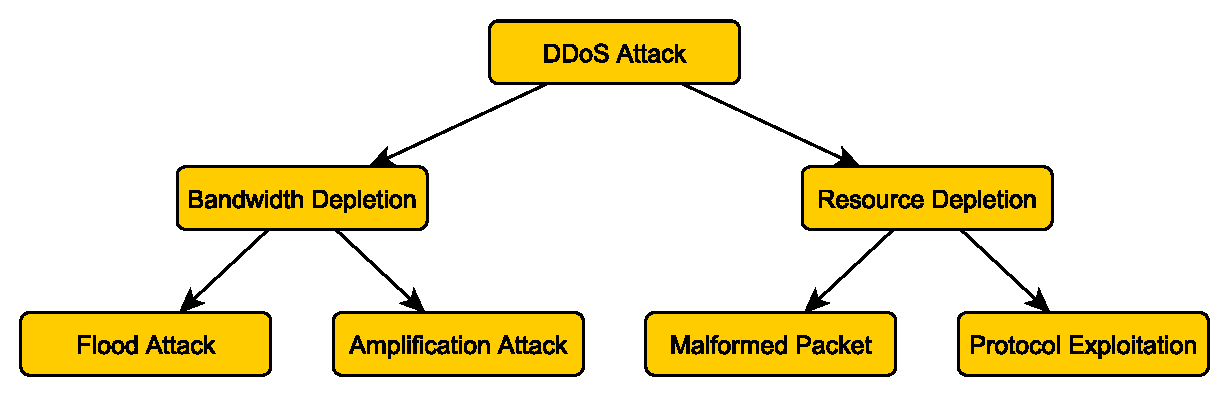
\includegraphics[width=\columnwidth]{section_2/DDoS_Taxonomy.eps}
    \caption{\gls{ddos} attack taxonomy  \cite{specht2004distributed}}
    \label{fig:Chap2_DDoS_Tax}
\end{figure}

Bandwidth depletion aims to deplete the network related resources of the victim. These attacks tend to generate large volumes of network traffic to deplete the bandwidth allocated to the victim's system. Resource depletion attacks aim to deplete the victim server's available resources rather than bandwidth.

Traditional amplification attacks leverage broadcast IP addresses to generate sufficient traffic to saturate the victim's bandwidth. The Smurf attack is an example of an amplification attack. The Smurf works by spoofing the IP address of the intended victim and then sending a ICMP\_ECHO\_REQUEST packet to a broadcast IP. The broadcast IP will broadcast the message to all the nodes within it's subnet, causing and amplification attack. The responses generated by the nodes, saturate the bandwidth of the victim server  \cite{kumar2007smurf}. According to Martin \textit{et al.}\cite{martin2002router} routers (as of 1999) no longer forward packets directed at their broadcast addresses. This means that most modern networks should be immune to Smurf attacks.

A \gls{drdos} attack is a modern variant of amplification attacks which uses vulnerable protocols or methods within protocols to generate large volumes of response traffic from legitimate service providers. This type of attack spoofs the IP address of the intended victim and performs a service request to the service provider using the spoofed IP address of the intended victim. The attack is known as a reflective attack because the response is ``reflected'' back to the victim IP address.  The \gls{udp} transportation layer protocol is often used to perform \gls{drdos} attacks due to lack of verification handshake in the \gls{udp} protocol  \cite{USCert2018}. By spoofing the IP address of the intended victim, neither the victim nor the service provider knows the true IP address of the attacker  \cite{USCert2018}.

An example of a \gls{drdos} attack is \gls{ntp} amplification. \gls{ntp} is an Internet protocol which is used to synchronise various web servers  \cite{RFC5905}.  The \gls{ntp} protocol has a method called $mon\_getlist$. By calling this method using the \gls{ntp} protocol, the service provider will respond with a list of \gls{ntp} response messages. The network traffic generated to make the $mon\_getlist$ request is significantly lower than the network traffic generated as a response \cite{czyz2014taming}. This is known as the amplification factor. Table~\ref{tab:2Amplify} provides the amplification factor for various protocols \cite{USCert2018}.

\begin{table}[h]
\centering
\caption{Amplification factor of various \gls{drdos} attacks \cite{USCert2018}}
\label{tab:2Amplify}
\begin{tabular}{| l | c | l | c |}
\hline
\textbf{Protocol}                                              & \textbf{\begin{tabular}[c]{@{}l@{}}Amplifica- \\ tion Factor\end{tabular}} & \textbf{Protocol}                                                & \textbf{\begin{tabular}[c]{@{}l@{}}Amplifica- \\ tion Factor\end{tabular}} \\ \hline
DNS                                                            & 28-54                                                                 & NTP                                                              & 556.9                                                                    \\ \hline
SNMPv2                                                         & 6.3                                                                      & NetBIOS                                                          & 3.8                                                                      \\ \hline
SSDP                                                           & 30.8                                                                     & CharGen                                                          & 358.8                                                                    \\ \hline
QOTD                                                           & 140.3                                                                    & Bit Torrent                                                      &                 3.8                                                         \\ \hline
\begin{tabular}[c]{@{}l@{}}Multicast DNS\\ (mDNS)\end{tabular} & 2-10                                                                  & \begin{tabular}[c]{@{}l@{}}Quake Network\\ Protocol\end{tabular} & 63.9                                                                     \\ \hline
Steam Protocol                                                 & 5.5                                                                      & Kad                                                              & 16.3                                                                     \\ \hline
RIPv1                                                          & 131.24                                                                   & \begin{tabular}[c]{@{}l@{}}Portmap\\ (RPCbind)\end{tabular}      & 7-28                                                                  \\ \hline
LDAP                                                           & 46-55                                                                 & CLDAP                                                            & 56-70                                                                 \\ \hline
TFTP                                                           & 60                                                                       & Memcached                                                         & \begin{tabular}[c]{@{}l@{}}10 000-\\ 51 000\end{tabular}               \\ \hline
\end{tabular}
\end{table}

At the time of writing this paper, the Memcached protocol produces the largest amplification factor of all known vulnerable protocols, see Table~\ref{tab:2Amplify} for full list of known vulnerable protocols and their corresponding amplification factors. According to the US \gls{cert}  \cite{USCert2018}, Memcached  has an amplification factor of 10 000 to 51 000, this means that for every byte of data sent by the attacker, the Memcached service responds with between 10 to 51 kilobytes of data. A high amplification factor greatly reduces the number of bots required by the attacker to launch a successful \gls{ddos} attack. 

Memcached is a network service which allows network
applications to cache database query results on networked
host, similar to how a computer's cache memory stores data in a temporary cache
 \cite{fitzpatrick2004distributed}. Memcached operates on \gls{udp} port 11211. The Memcached service allows distributed clusters of computers to store frequently requested database query results on the Memcached server rather than requiring additional database look-ups to retrieve the data. Depending on the Memcached server setup large volumes of data can be stored in the Memcached cache. It is best practise to not allow Memcached servers to be accessable from outside an organisation's firewall as the Memcached service may expose sensitive data over the network  \cite{ranabahu2009best}. Unfortunately due to misconfiguration or neglect of best practises some Memcached services are exposed to the Internet.  

During a \gls{drdos} attack, the attacker spoofs the IP address of the intended victim. Using the spoofed address, the attacker, requests that a large portion (if not all) of the data stored within the Memcached cache be returned as a result to the spoofed IP address. This results in the victim machine receiving a large volume of unsolicited network traffic.  If the attacker performs enough requests on behalf of the victim, the victims network resources will become depleted and prevent the victim from delivering services to legitimate network users. 

In the next Section, the data collection environment used to detect and mitigate the Memcached attack will be discussed.



 